\documentclass[11pt]{report}
\usepackage{StyleSheets/main}
\begin{document}

\chapter{Conceptual Design}\label{ch:conceptual-design}

\section*{Design Strategy}
Before the initial design process had begun, it was clear to the team that there would be a trade-off between complexity and efficiency --- as such, it was determined that the complexity of the system would have to increase greatly in order to get the maximum potential performance from the robot. The following designs are variations of the previous, with each design increasing in complexity.
\par Other teams reduced the amount of electrical components that connected to the Teensy 4.1 microcontroller to reduce the complexity of the code base, seen in \cref{ap:code}. This did not influence the design of this robot as the code base was designed from the ground up to be a modular system, utilizing an object oriented approach in \cplusplus{}, ensuring no extra code needed to be written or maintained the more sensors were added to the cart. Consequently, the design process was unrestricted by the quantity or variety of sensors available, permitting a more flexible approach to design.

\subsection*{Abbreviations used in Drawings}
\begin{itemize}
    \item \gls{US}
    \item \gls{CS}
    \item \gls{IRS}
    \item \gls{omni}
    \item \gls{FS}
    \item \gls{B}
\end{itemize}

\newpage
\section{Design 1}\label{sec:design1}
\begin{figure}[H]
    \centering
    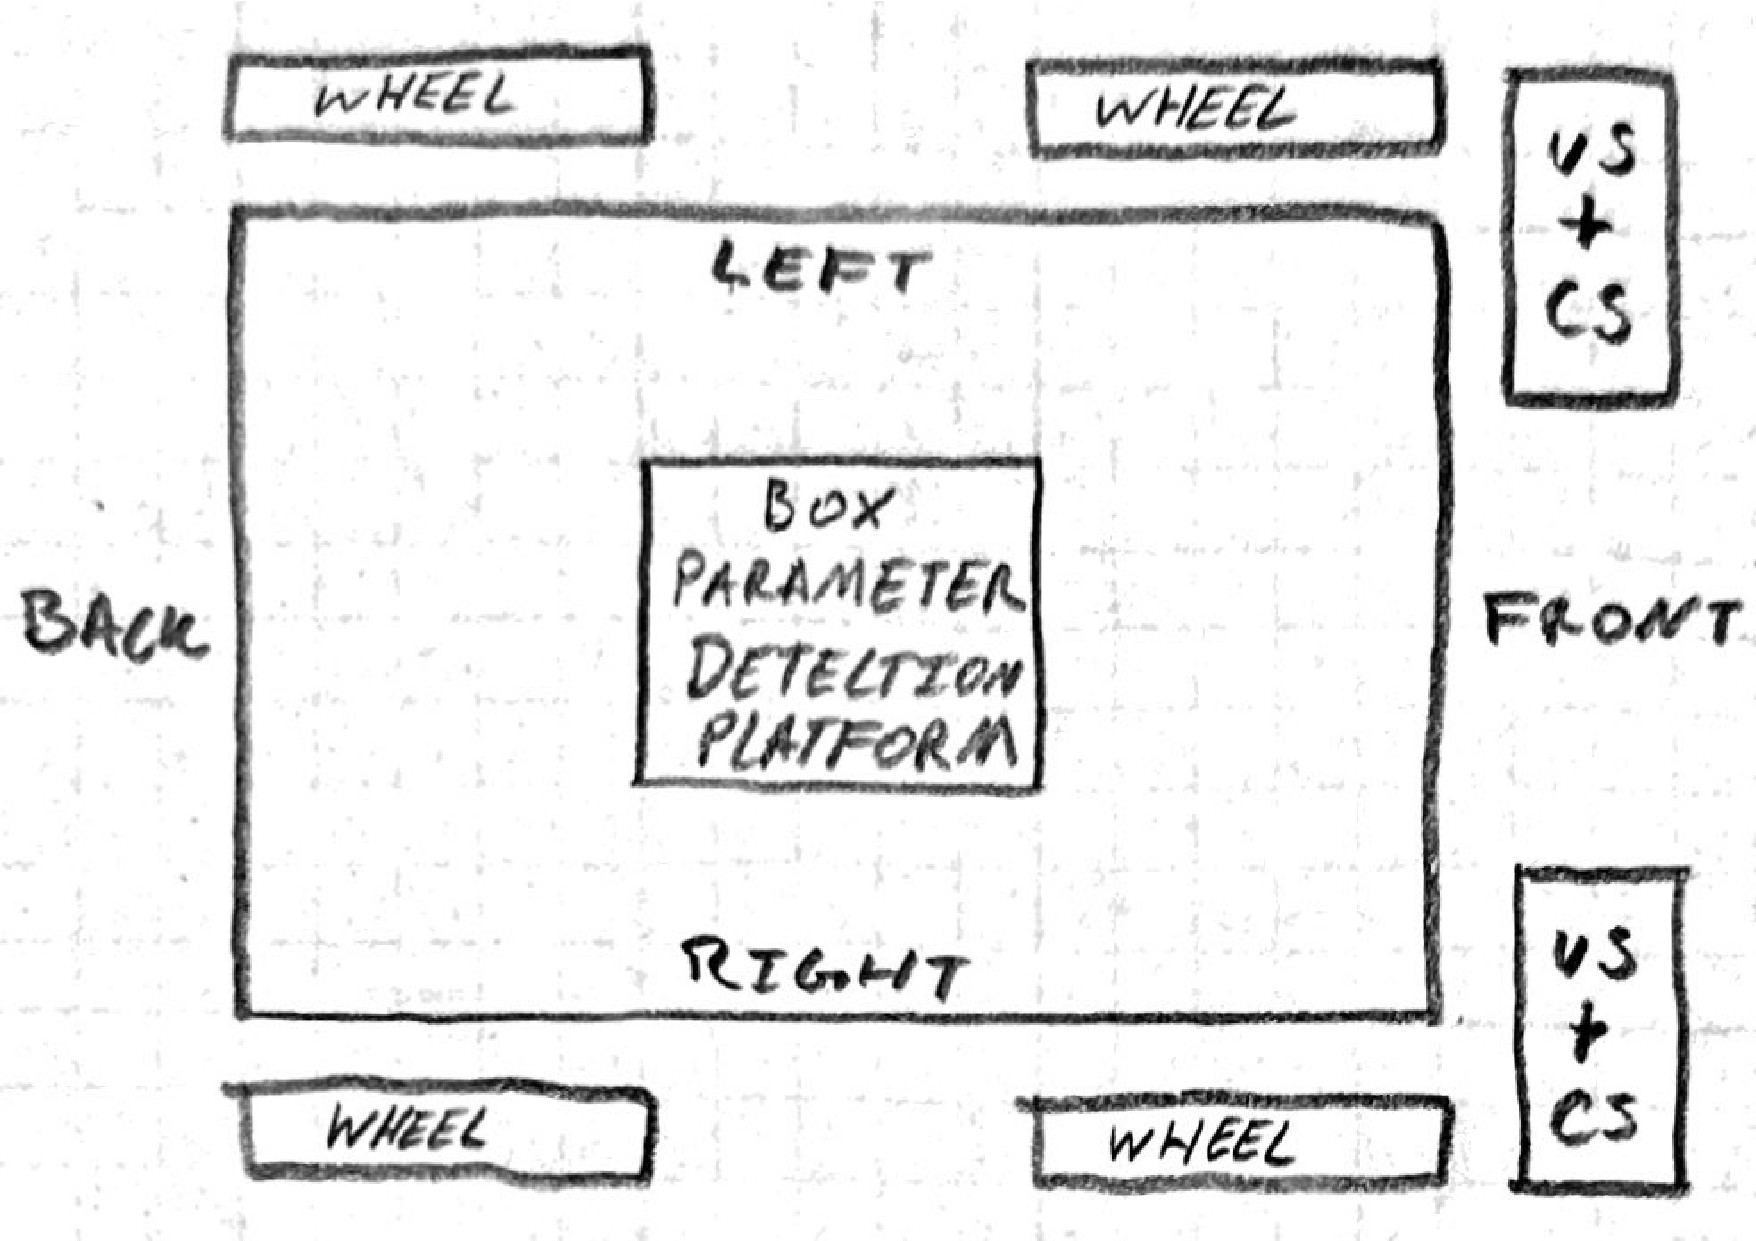
\includegraphics[width=0.5\linewidth]{Images//Designs/Design1a.pdf}
    \caption{Design 1a - simplified layout of movement and sensor systems}
    \label{fig:design1a}
\end{figure}
The first design is an adaptation of the fundamental designs demonstrated throughout the prerequisite course, Integration I, for the sake of setting a baseline. Efficiency and speed are sacrificed for simple movement and sensor algorithms.

\begin{description}
    \item[Wheel Configuration --] This design utilizes a standard 2x2 wheel configuration featuring standard 1 \gls{DoF} wheels. This configuration performed consistently, yet was problematic when it came to creating highly dynamic movement algorithms.
    %
    \item[Sensor Configuration --] The front corners are fitted with dual-purpose sensor mounts, containing both an \gls{RGB} color sensor and an ultrasonic sensor to be used for all spatial objectives: line following, boundary/obstacle/object detection, and directional orientation.
\end{description}

\begin{figure}[H]
    \centering
    \hspace*{6em}
    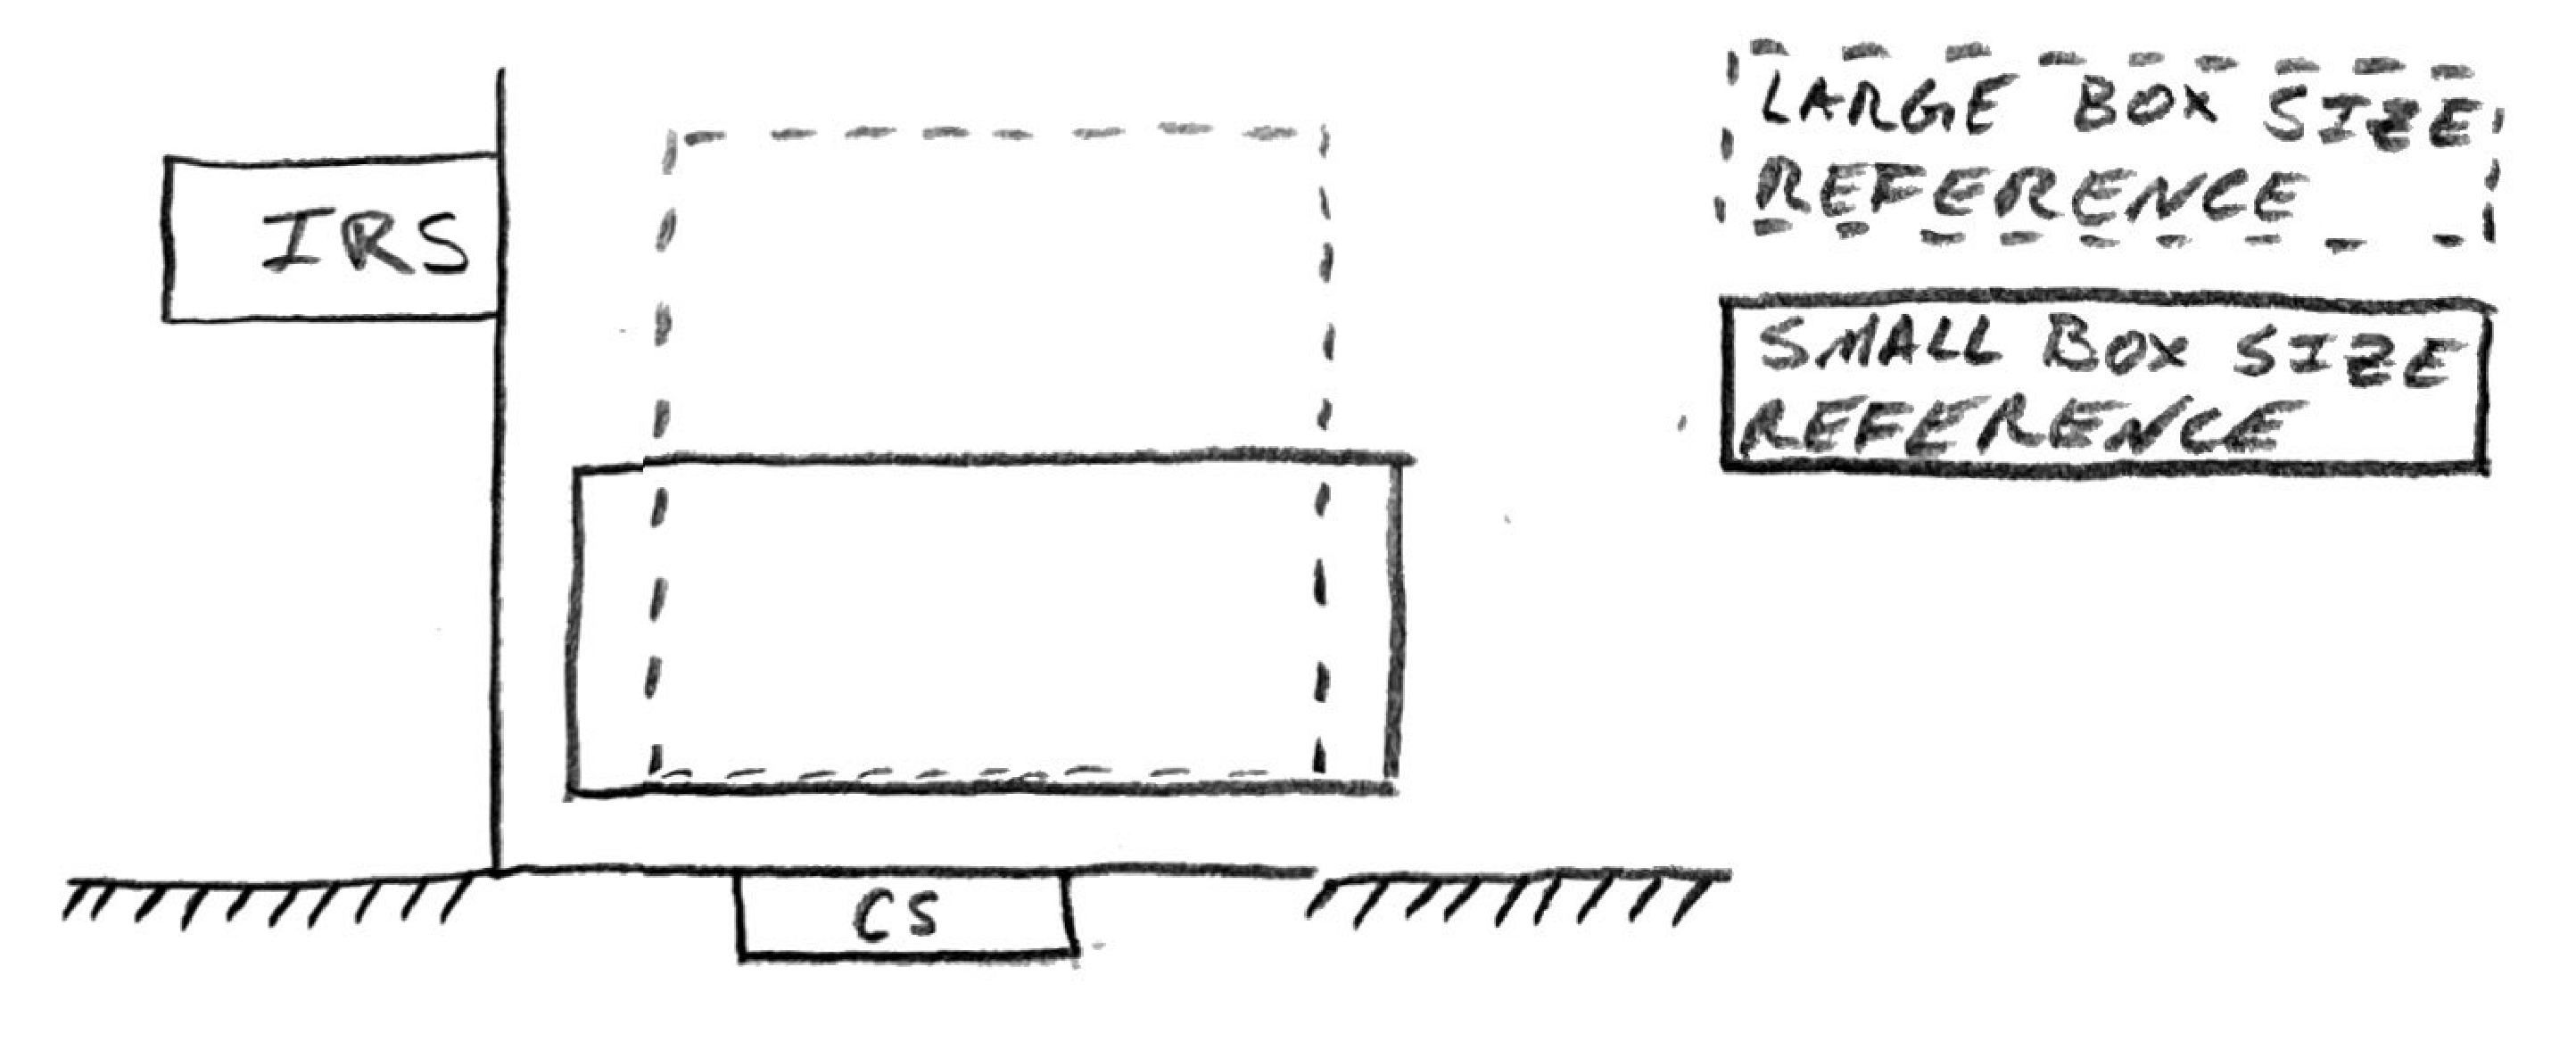
\includegraphics[width=0.6\linewidth]{Images//Designs/Design1b.pdf}
    \caption{Design 1b --- Box property detection platform with IRS}
    \label{fig:design1b}
\end{figure}
\begin{description}
    \item[Box Property Detection --]A gripper mechanism is to place the box onto a small platform on top of the robot that will contain an \gls{RGB} sensor to determine the package color, alongside an infrared sensor placed high enough to only detect the larger of two possible box sizes.
\end{description}

\newpage
\section{Design 2}\label{sec:design2}
\begin{figure}[H]
    \centering
    \hspace*{2em}
    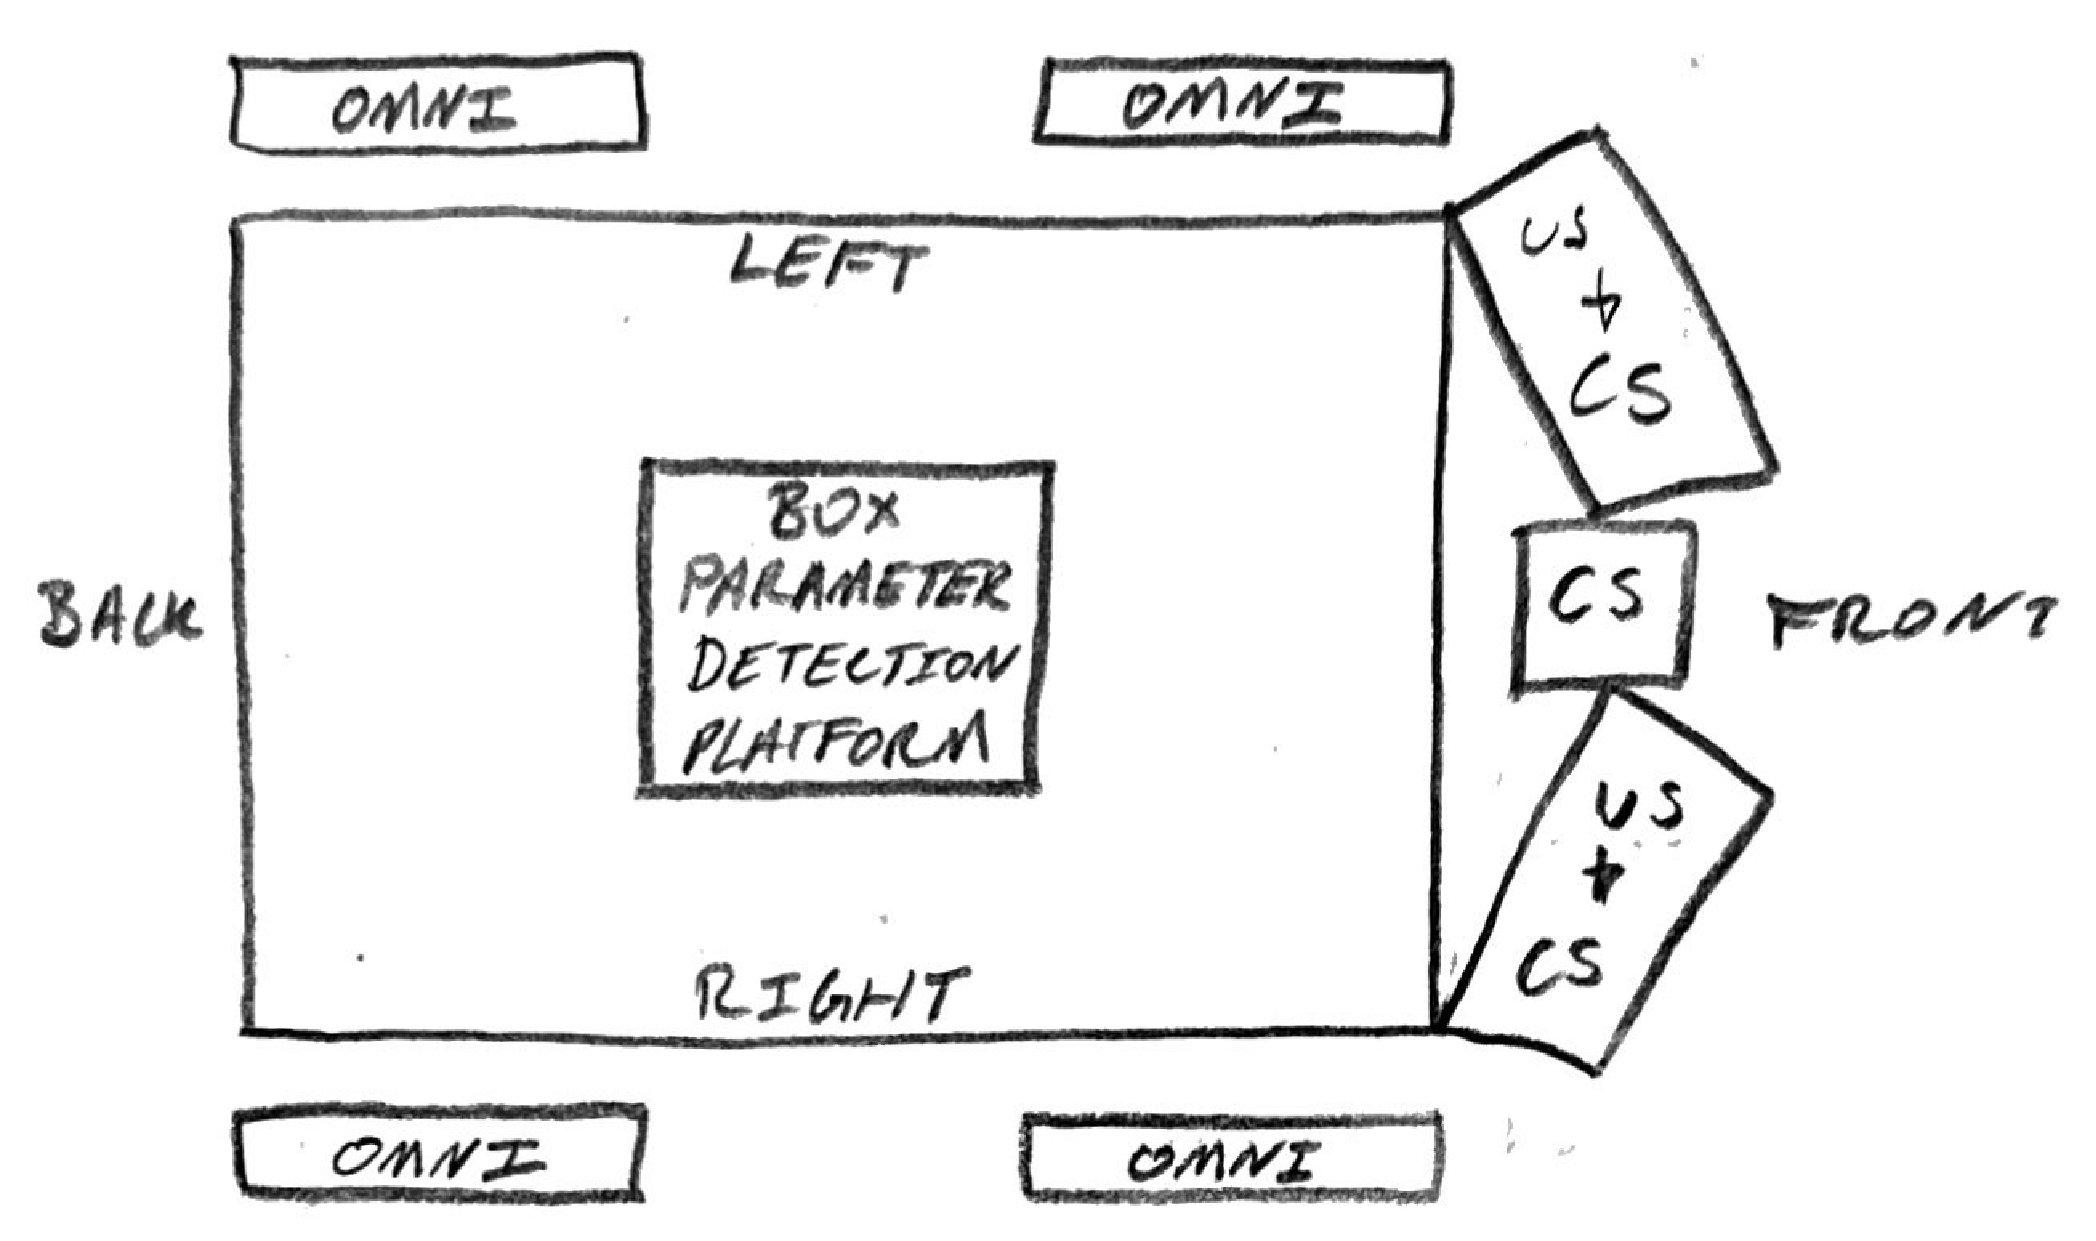
\includegraphics[width=0.5\linewidth]{Images//Designs/Design2a.pdf}
    \caption{Design2a --- simplified layout of movement and sensor systems}
    \label{fig:design2a}
\end{figure}
The second design functions nearly identically to \cref{sec:design1} but with minor alterations to the sensor layout, as well as the introduction of \gls{omni}-wheels.

\begin{description}
    \item[Wheel Configuration --] This design still utilizes a standard 2x2 wheel configuration, but instead utilizes \gls{omni}-wheels with 2 \gls{DoF}. The implementation of \glspl{omni} fixes some of the aforementioned problems with dynamicism by enabling the robot to pivot more easily and with more control.
    %
    \item[Sensor Configuration --] This iteration uses a similar sensor layout to the previous, but this time the ultrasonic sensors are angled outward slightly, in theory, reducing the time it takes to identify objectives, subsequently increasing the overall efficiency of the system. Additionally, a third color sensor is attached to the center of the robot to increase the available information during line following functions.
\end{description}

\begin{figure}[H]
    \centering
    \hspace*{6em}
    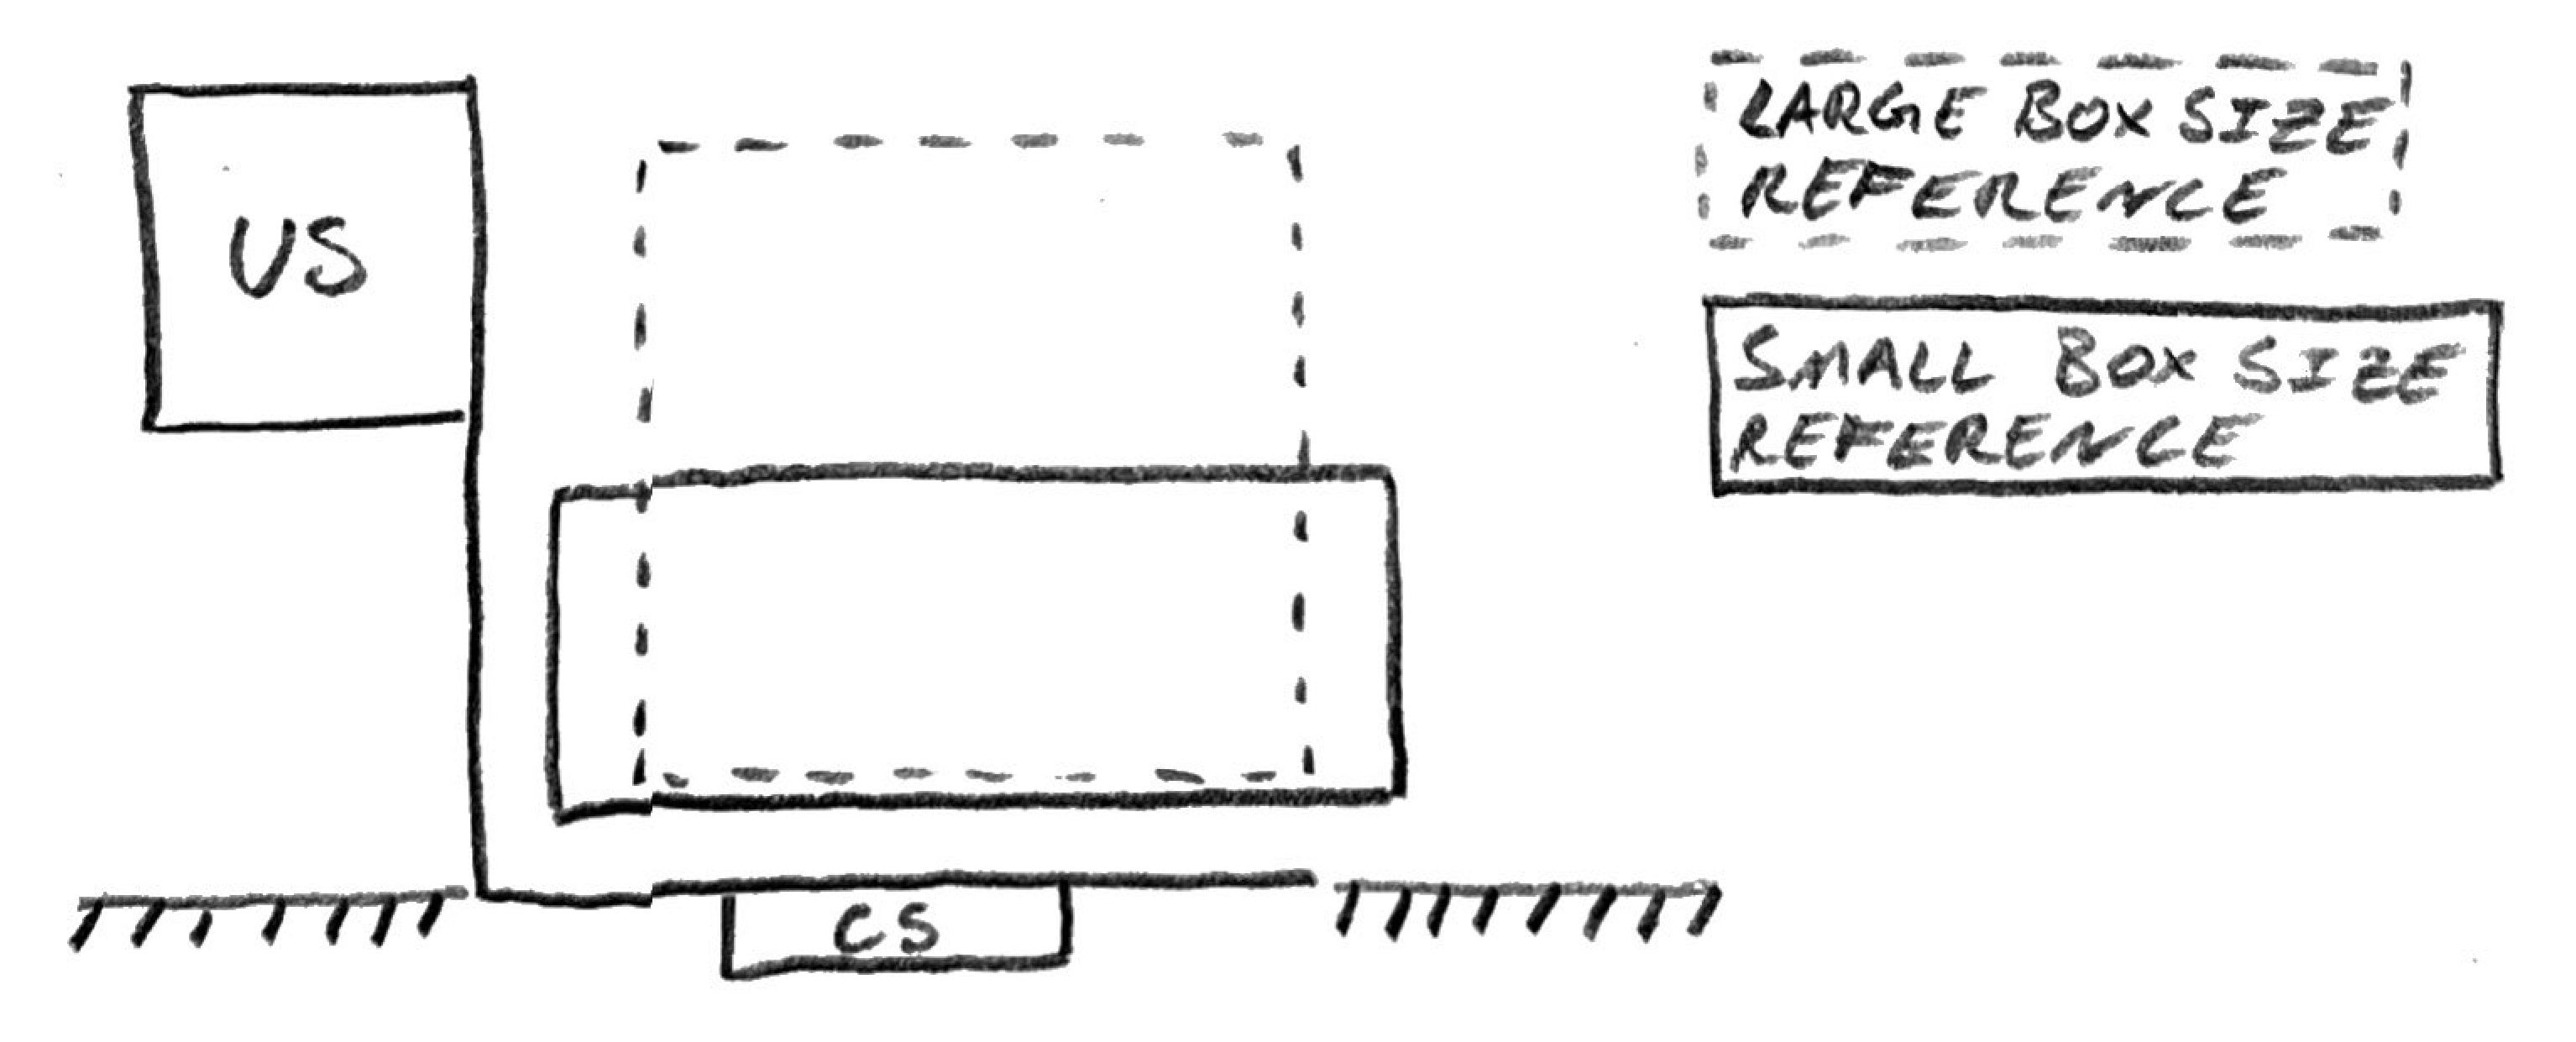
\includegraphics[width=0.6\linewidth]{Images//Designs/Design2b.pdf}
    \caption{Design 2b --- Box property detection platform with IRS}
    \label{fig:design2b}
\end{figure}
\begin{description}
    \item[Box Property Detection --]Again, a gripper mechanism places the box onto a platform that will then determine the properties of the package. An \gls{RGB} sensor is still used to get the color of the box, but an ultrasonic sensor replaces the \gls{IR} sensor. It should be noted that the swap from \gls{IRS} to \gls{US} was simply to provide another option during testing and assembly; there is no immediately identifiable benefit to using one over the other.
\end{description}

\newpage
\section{Design 3}\label{sec:design3}
\begin{figure}[H]
    \centering
    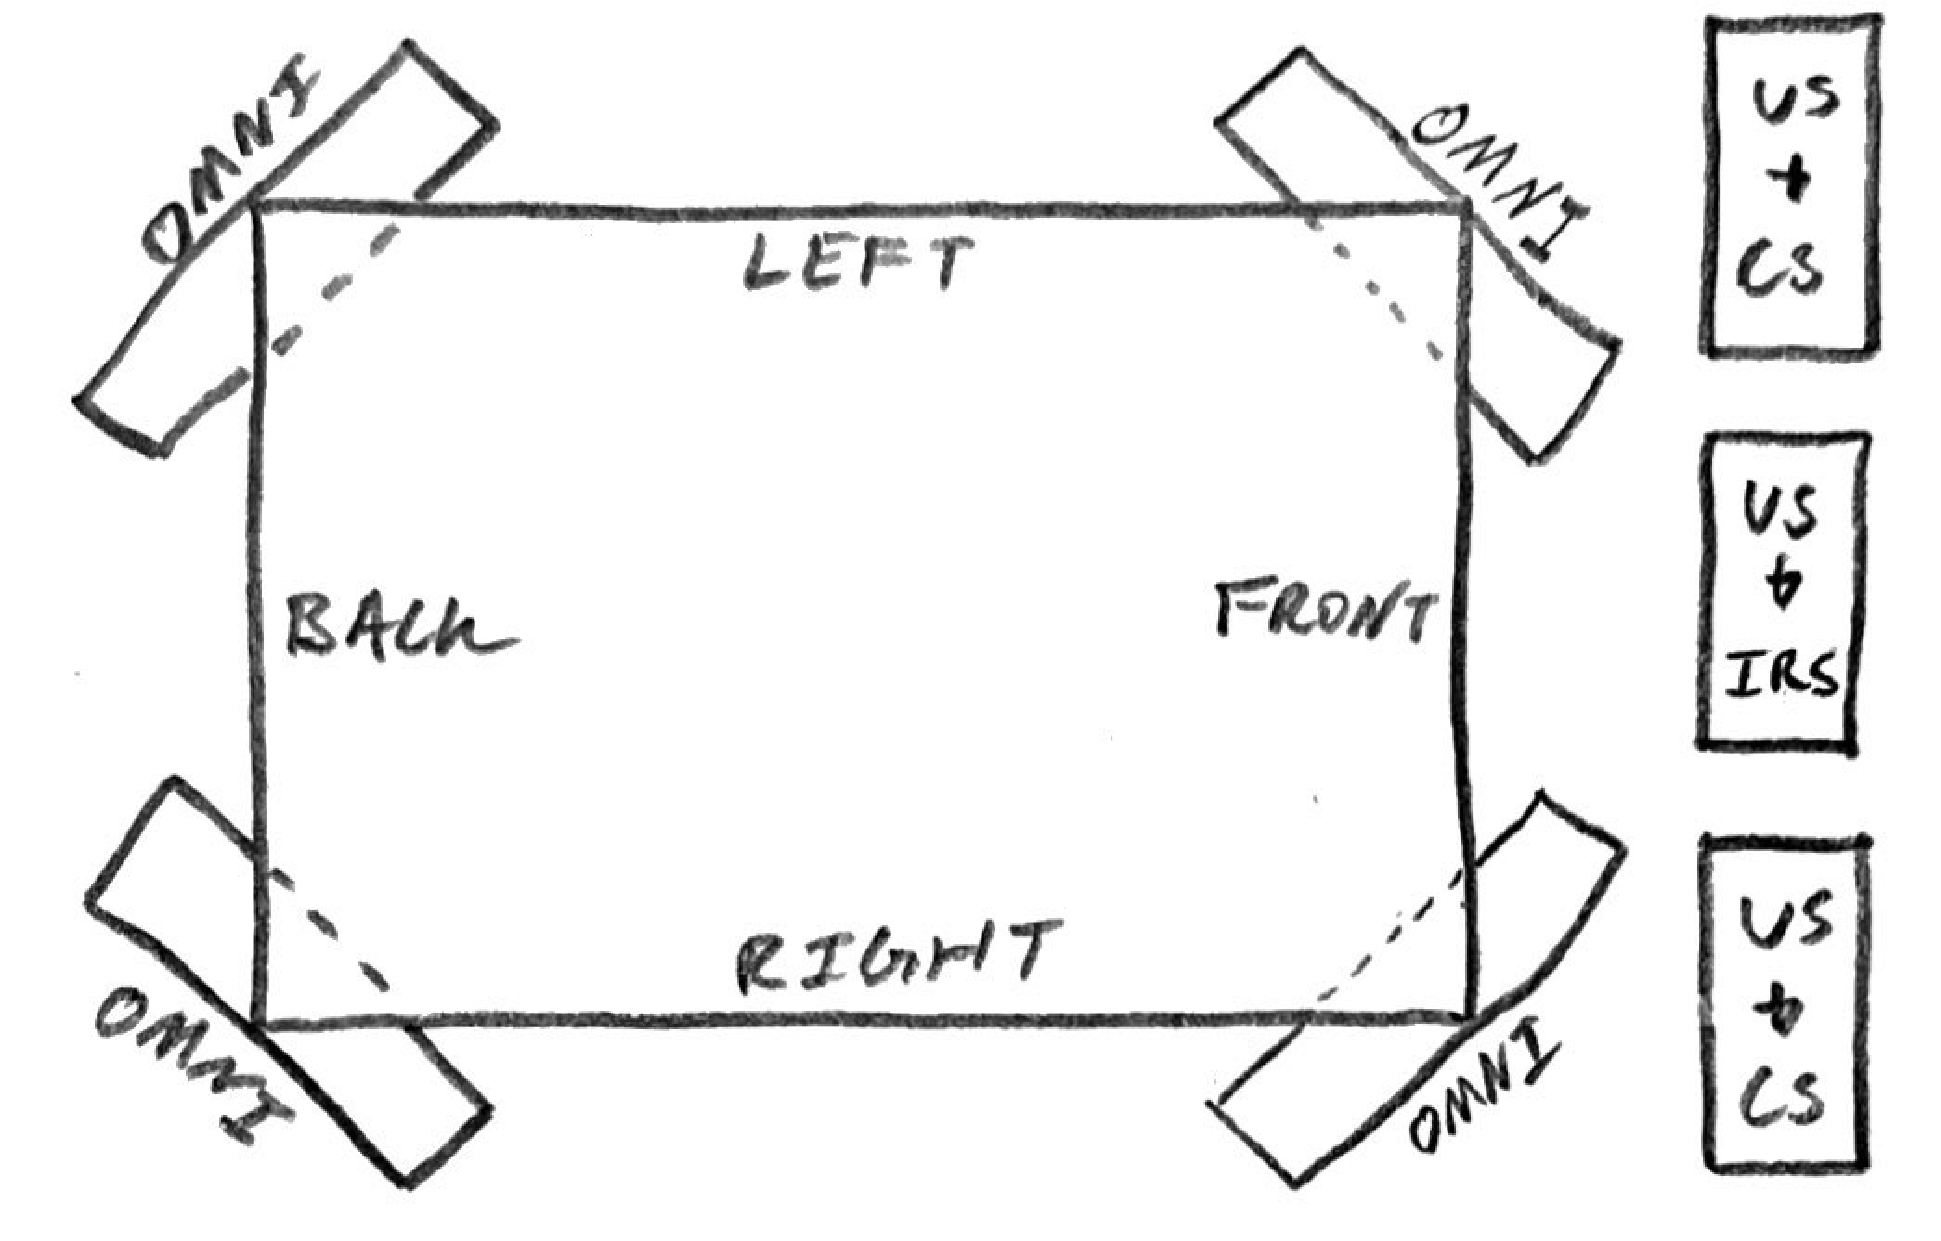
\includegraphics[width=0.5\linewidth]{Images//Designs/Design3a.pdf}
    \caption{Design 3a --- simplified layout of movement and sensor systems}
    \label{fig:design3a}
\end{figure}
The third design introduces a new movement strategy, and features a new sensor layout intended for smarter movement capabilities.
\begin{description}
    \item[Wheel Configuration --]The \glspl{omni} are now placed in a cornered configuration to enable crab-walking: linear translation in cardinal directions, or otherwise, via relative \gls{PWM} control.
    \item[Sensor Configuration --]The ultrasonic sensors on the sides have been reverted to the original forward-facing orientation due to the addition of a third ultrasonic sensor. The side ultrasonic sensors are intended to be in-line with the wheels to predict possible collisions across the whole robot, and the centrally located one allows for faster targeting of the pick-up-and-place platforms. Lastly, two or more centered \gls{IR} sensors are utilized for line-following purposes.
\end{description}
\begin{figure}[H]
    \centering
    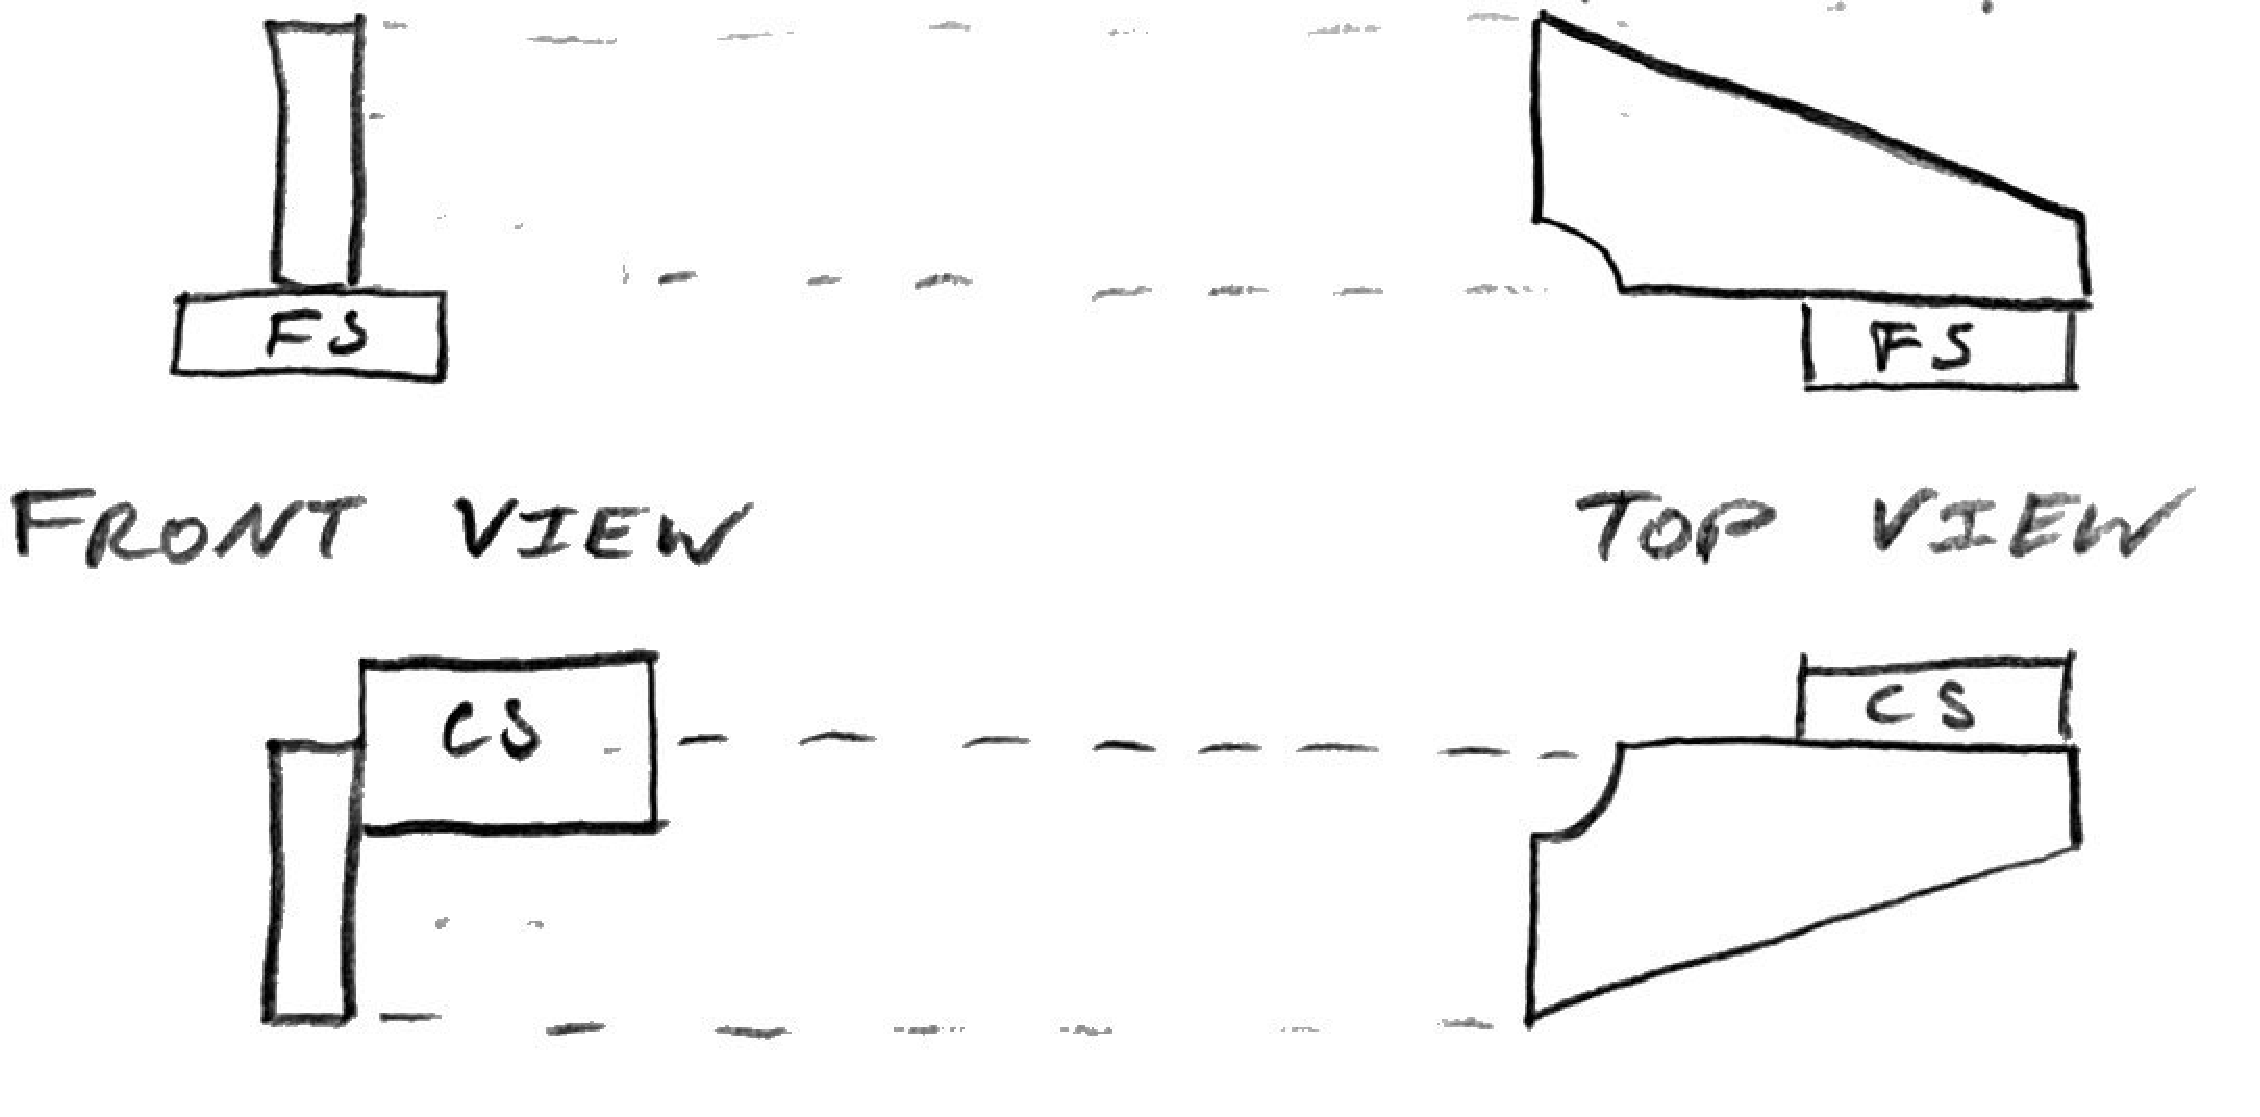
\includegraphics[width=0.5\linewidth]{Images//Designs/Design3b.pdf}
    \caption{Design 3b --- Box property detection platform with IRS}
    \label{fig:design3b}
\end{figure}
\begin{description}
    \item[Box Property Detection --]This iteration removes the property detection platform entirely and includes all relevant sensors on the gripper itself via 3D printed mounts. The color sensor will be mounted on one mandible, while a force-sensor, denoted \gls{FS}, using a timing-based algorithm to determine box size will be placed on the other.
\end{description}

\newpage
\section{Design 4}\label{sec:design4}
\begin{figure}[H]
    \centering
    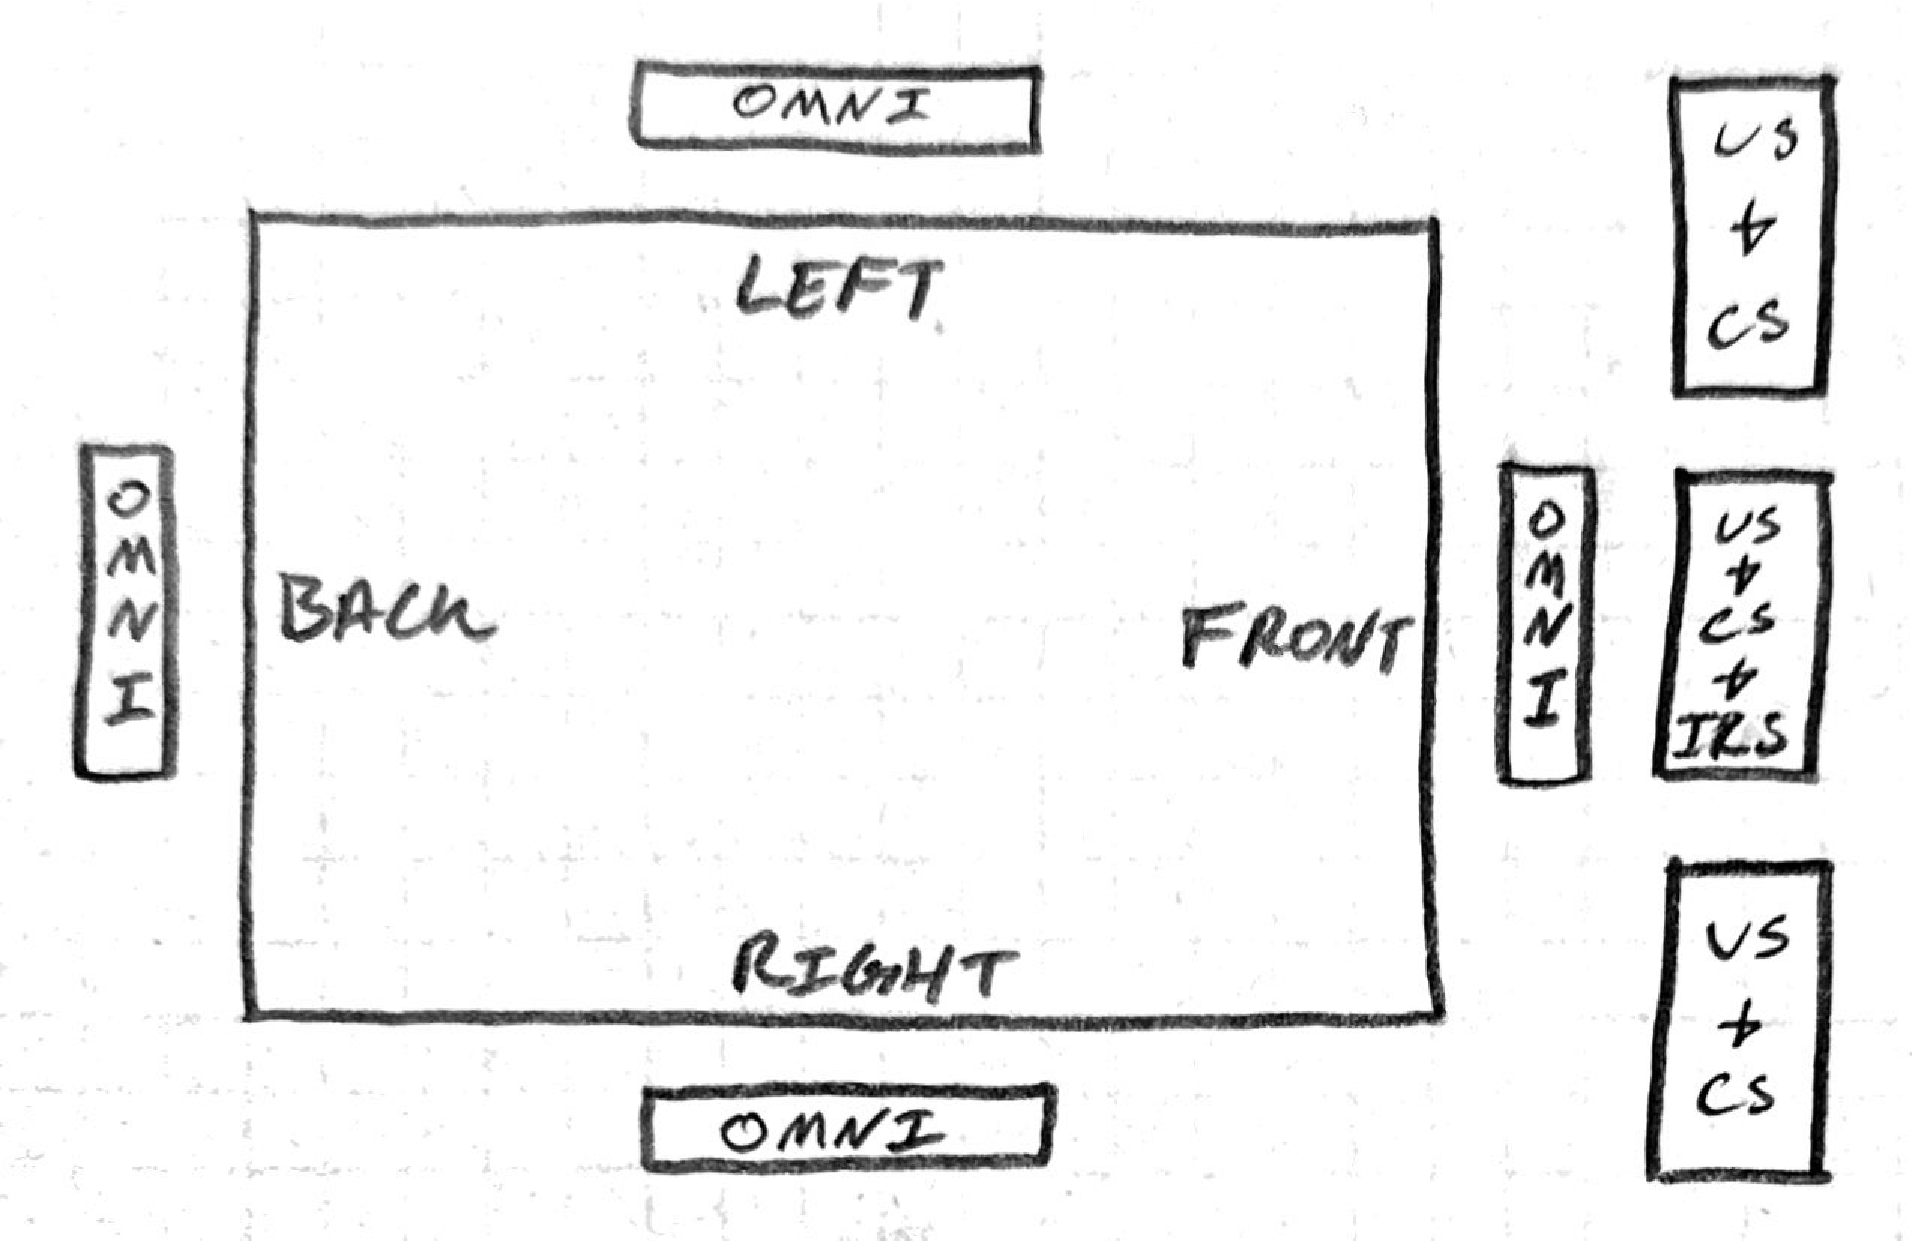
\includegraphics[width=0.5\linewidth]{Images//Designs/Design4a.pdf}
    \caption{Design 4a --- simplified layout of movement and sensor systems}
    \label{fig:design4a}
\end{figure}
The fourth design reorients the wheels as to be square against the sides, and combines the ideas for centralized sensors of \cref{sec:design2} and \cref{sec:design3}. This was chosen as the final design; the decision matrix supporting this design ca
\begin{description}
    \item[Wheel Configuration --]The \glspl{omni} are now placed in a squared configuration to increase the maximum speed potential, as the cornered configuration has inherent losses in the cardinal directions --- those most relevant to the tasks presented.
    \item[Sensor Configuration --]This iteration uses the middle color sensor idea from \cref{sec:design2}, and the centralized \gls{IR} array and ultrasonic sensor from \cref{sec:design3}. Together, these sensors provide as much information about the robot's location and orientation as possible.
\end{description}
\begin{figure}[H]
    \centering
    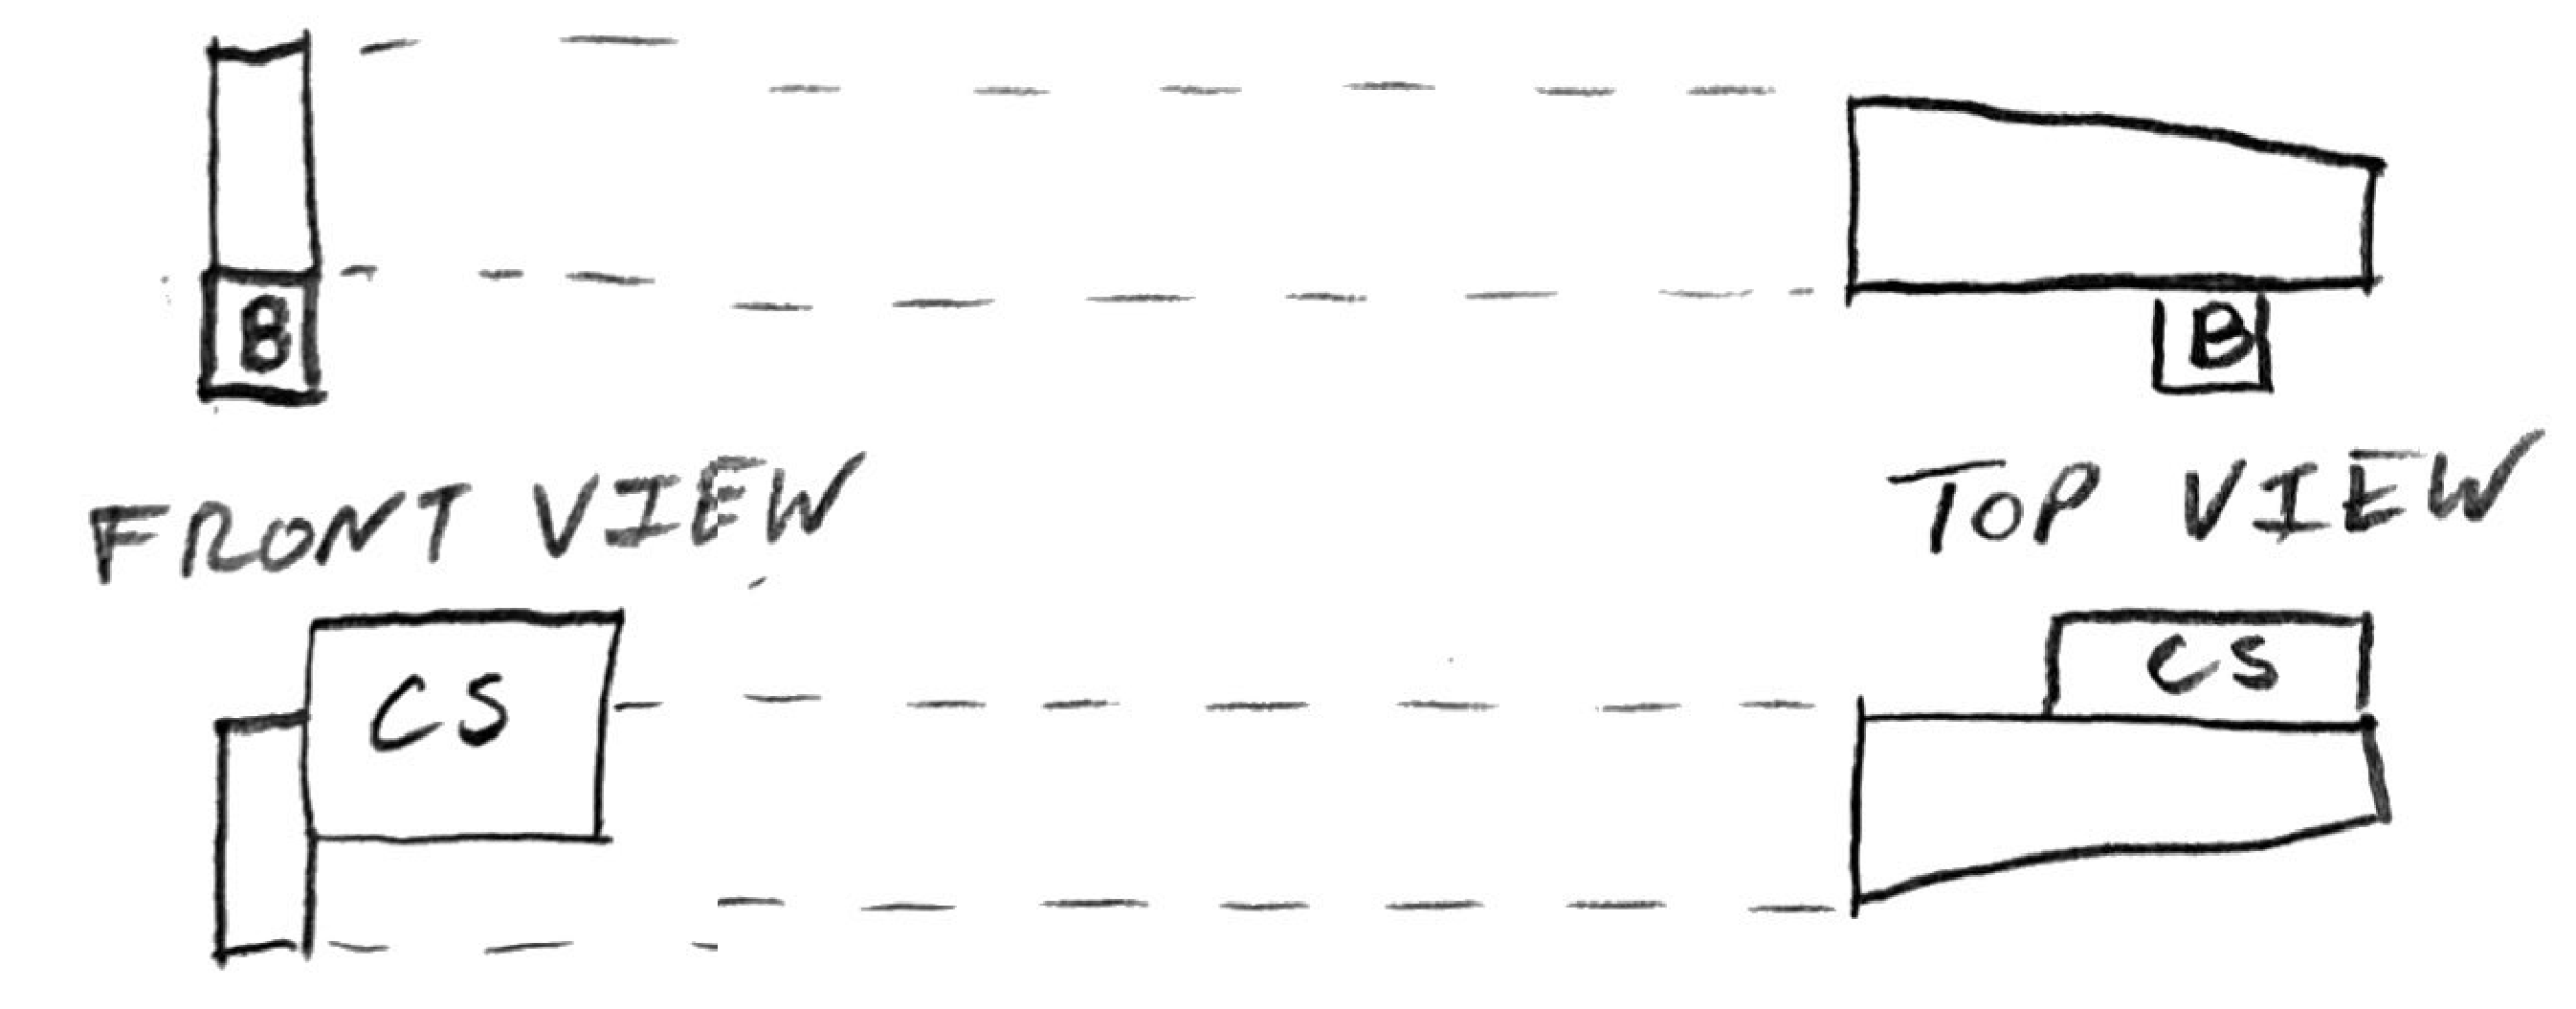
\includegraphics[width=0.5\linewidth]{Images//Designs/Design4b.pdf}
    \caption{Design 4b --- Box property detection platform with IRS}
    \label{fig:design4b}
\end{figure}
\begin{description}
    \item[Box Property Detection --]This gripper sensor layout is identical to the last with a button, denoted \gls{B}, in place of the force sensor, which will operate under a similar algorithm while eliminating the inconsistency of the force sensor.
\end{description}

\end{document}